\chapter{Szimulációs és validációs keretrendszer}
\section{Elvárások az alkalmazással szemben}

%TODO Itt kellene röviden áttekinteni az alkalmazással szemben támasztott követelményeket.
Az alkalmazás legfőbb feladata egy konverzió elvégzése BPEL és Petri-háló modellek között. Ebből adódóan minden BPEL elemet le kell tudnia kezelni, illetve az azok közti összefüggéseket feltérképezi, és az összefüggés halmazból egy Petri-hálót előállítani. A rendszer a hálót felépíti, valamint a hálón belüli mozgásokat rajzolja, és szükségesség esetén input file-t vagy felhasználói inputot kezel. Ha a háló nem hozható létre, akkor azt tudatnia kell, és lehetőség szerint rövid indoklással alátámasztania. 

\section{Az alkalmazás felépítése}

%TODO Osztály és blokkdiagramok formájában be kellene mutatni, hogy milyen fő elemekből épül fel az alkalmazás.
Az alkalmazás logikailag a következő fő részekből áll:
\begin{itemize}
\item I/O module: Beolvassa az XML dokumentumot és értelmezi. Szükség esetén menti a kész hálót.
\item Conversion module: Átkonvertálja  a beolvasott dokumentumot.
\item Data Structure module: A saját típusú Petri elemeket kezeli, és adatszerkezeti implementációt tartalmaz. 
\item UI talker: A UI ra illeszti a megfelelő input mezőt, az abba felvitt értéket átadja a feldolgozó egységnek.
\item Graphics module: Az MSGL libraryre épül. Feladata a gráf rajzolása és megjelenítése animációval együtt. 
\item Computing module: A háló animációjához végzi a szükséges számításokat és időzítéseket. 
\end{itemize}
A programmodulok pedig a következők:
\begin{itemize}
\item Form: Az alkalmazás layoutját tartalmazza, illetve a rajta levő elemekhez rendelt kódot. (pl, gombok függvényhívását, töltődési inicializációt, stb.)
\item GraphBuilder: A petri hálót (mint gráfot) generálja. Saját leíró nyelvet használ, a Model-ben levő hálóz veszi alapul.
\item Model: Tartalmazza a Petri háló és elemeinek leírását, valamint az MASGL saját node alapú architektúra definíciót, a könnyebb generálás érdekében.
\item Resources: A projekt által használt "erőforrásokat" ide tartoznak a tesztelési adatstruktúrák, bemenetek, illetve a különböző placeholder képek. 
\item XmlHandler: Az BPEL (xml) fileok beolvasását és parse-olását ahjtja végre. Kimenete egy feltérképezett XML struktúra, amiben majdnem azonnal lehet különböző node-okra ugrani. 
\item Converter: A különböző adatstruktúrák közötti konverziós logikát tartalmazza, a segéd adatstruktúrákkal. 

\begin{figure}[h!]
\centering
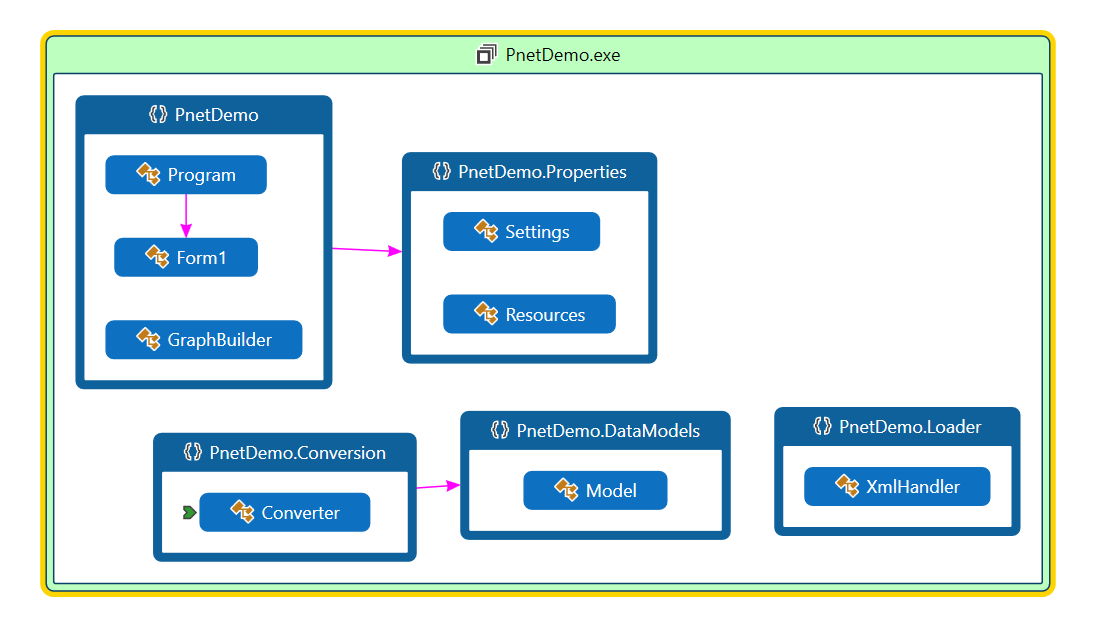
\includegraphics[scale=0.5]{images/Classdiagram.png}
\caption{Az alkalmazás osztálydiagrammja  }
\label{fig:assign}
\end{figure}


\end{itemize}
